\begin{problem}
{\textbf{\textsc{Liquid Lenses}}} A large cylindrical well, with a radius of 1 meter and a depth much greater than the radius ($d \gg r$), is filled with reflective liquid metal. The well and the liquid within it is then set into rotation around its central axis at an angular speed of $\omega = 5\;\mathrm{rad/s}$, causing the edge of the liquid surface to rise and touch the brim of the well. Positioned directly above the well is a circular lamp with a radius of $1\;\mathrm{m}$, emitting photons vertically downward at a uniform rate and density. If the rate at which photons leave the lamp is $r$, then the rate at which photons collide with the liquid metal can be expressed as $nr$, where $n$ is a dimensionless constant. What is the value of $n$?
% \FloatBarrier 
% \begin{figure}[!htbp]
%      \centering
%     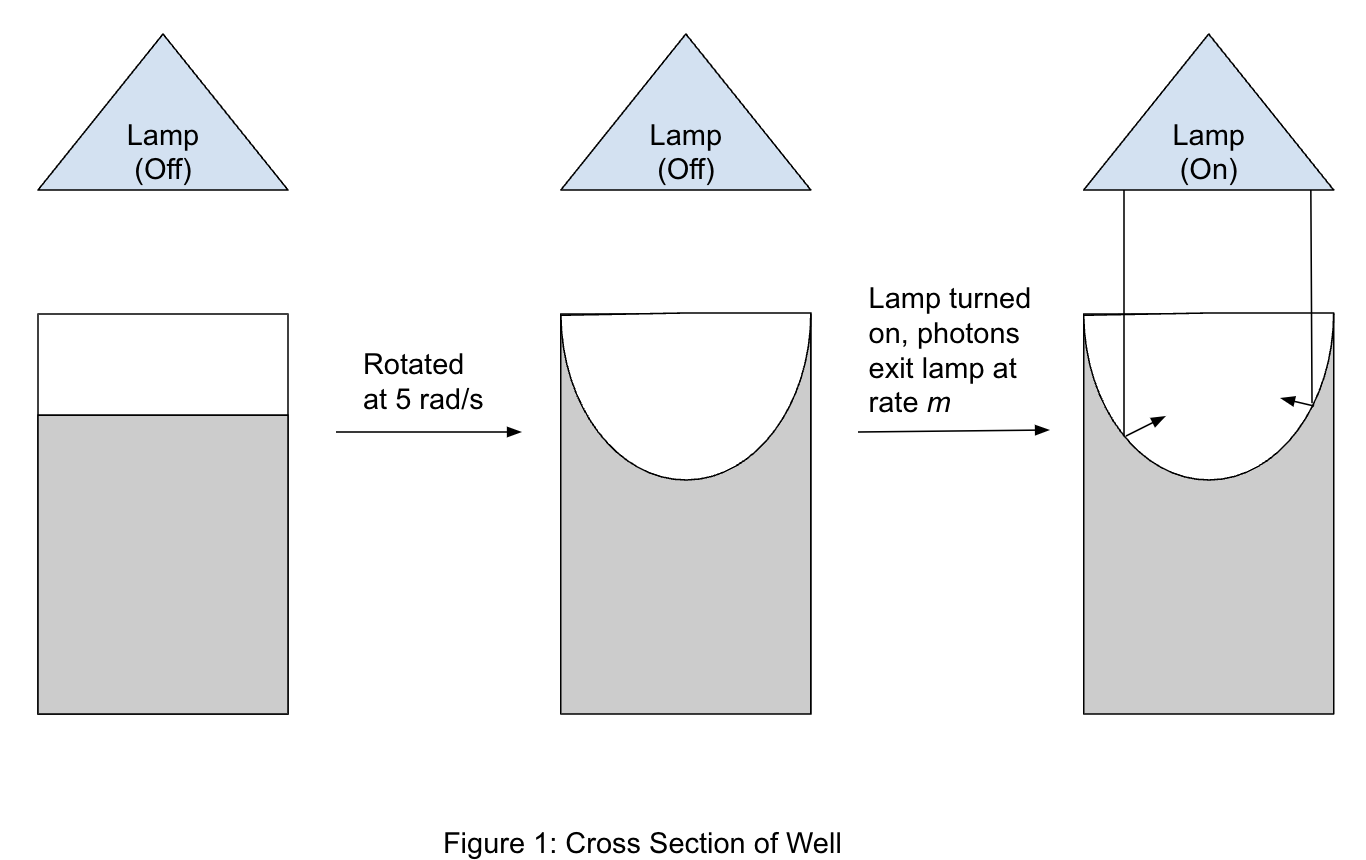
\includegraphics[scale=0.42]{problems/figures/wellDiagram.png}
%  \end{figure}
% \FloatBarrier

\end{problem}